% This LaTeX was auto-generated from MATLAB code.
% To make changes, update the MATLAB code and export to LaTeX again.

\documentclass{article}

\usepackage[utf8]{inputenc}
\usepackage[T1]{fontenc}
\usepackage{lmodern}
\usepackage{graphicx}
\usepackage{color}
\usepackage{hyperref}
\usepackage{amsmath}
\usepackage{amsfonts}
\usepackage{epstopdf}
\usepackage[table]{xcolor}
\usepackage{matlab}
\usepackage[paperheight=795pt,paperwidth=614pt,top=72pt,bottom=72pt,right=72pt,left=72pt,heightrounded]{geometry}

\sloppy
\epstopdfsetup{outdir=./}
\graphicspath{ {./clusterTSK_5mf_1order_media/} }

\begin{document}

\begin{par}
\begin{flushleft}
download of the dataset and verification of no correlation between the different features through a scatter plot of every feature with the others (could have done a confusion matrix too)
\end{flushleft}
\end{par}

\begin{matlabcode}
clear,close all;
data=load("airfoil_self_noise.dat");
% for i=1:5
%     for j=2:6
%         figure;
%         scatter(data(:,i),data(:,j));
%         title([num2str(i) "and" num2str(j)]);
%     end
% end
\end{matlabcode}

\begin{par}
\begin{flushleft}
let's see for clustering, here the elbow method, we can see the stagnation at 13 clusters
\end{flushleft}
\end{par}

\begin{matlabcode}
totaldistance=zeros(1,100);
for i=1:100
    [Kid,Kcenters,Kdsum]=kmeans(data,i);
    % Kdsum=Kdsum/max(Kdsum);
    for k=1:length(Kdsum)
        totaldistance(1,i)=totaldistance(1,i)+Kdsum(k);     
    end
end
figure;
plot(totaldistance);
title('Elbow method plot');
xlabel('Number of Clusters');
ylabel('Total distance from point to cluster')
\end{matlabcode}
\begin{center}
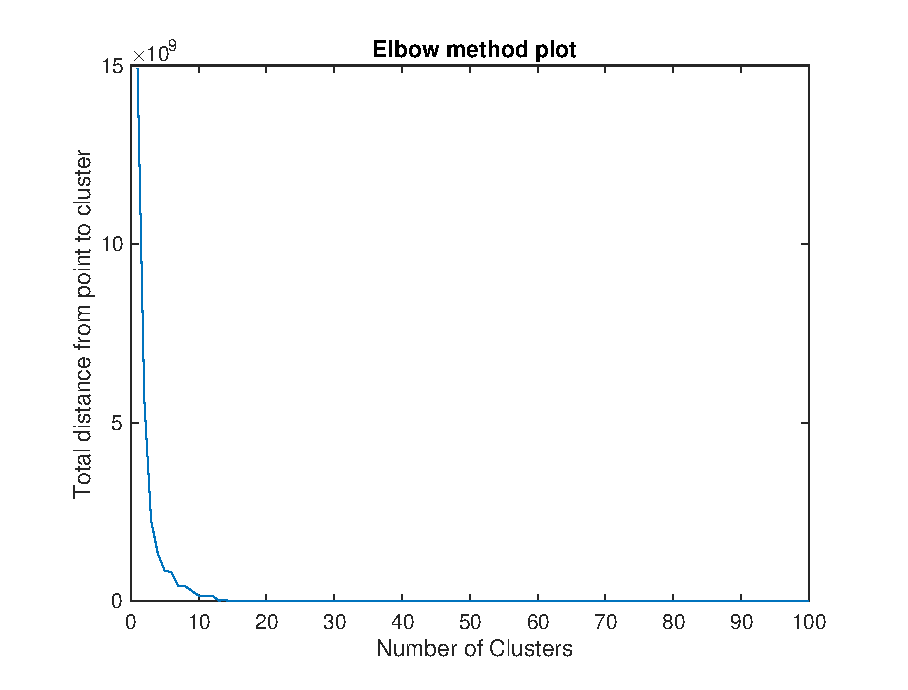
\includegraphics[width=\maxwidth{56.196688409433015em}]{figure_0.eps}
\end{center}
\begin{matlabcode}
max(data(:,1)) 
\end{matlabcode}
\begin{matlaboutput}
ans = 20000
\end{matlaboutput}
\begin{matlabcode}
min(data(:,1))
\end{matlabcode}
\begin{matlaboutput}
ans = 200
\end{matlaboutput}
\begin{matlabcode}
max(data(:,2)) 
\end{matlabcode}
\begin{matlaboutput}
ans = 22.2000
\end{matlaboutput}
\begin{matlabcode}
min(data(:,2))
\end{matlabcode}
\begin{matlaboutput}
ans = 0
\end{matlaboutput}
\begin{matlabcode}
max(data(:,3)) 
\end{matlabcode}
\begin{matlaboutput}
ans = 0.3048
\end{matlaboutput}
\begin{matlabcode}
min(data(:,3))
\end{matlabcode}
\begin{matlaboutput}
ans = 0.0254
\end{matlaboutput}
\begin{matlabcode}
max(data(:,4)) 
\end{matlabcode}
\begin{matlaboutput}
ans = 71.3000
\end{matlaboutput}
\begin{matlabcode}
min(data(:,4))
\end{matlabcode}
\begin{matlaboutput}
ans = 31.7000
\end{matlaboutput}
\begin{matlabcode}
max(data(:,5))
\end{matlabcode}
\begin{matlaboutput}
ans = 0.0584
\end{matlaboutput}
\begin{matlabcode}
min(data(:,5))
\end{matlabcode}
\begin{matlaboutput}
ans = 4.0068e-04
\end{matlaboutput}
\begin{matlabcode}

% for i=1:100
%     [c,u,obj]=fcm(data,i);
%     % Kdsum=Kdsum/max(Kdsum);
%     cost(i)=min(obj);
% end
% figure;
% plot(cost);
% title('Elbow method plot');
% xlabel('Number of Clusters');
% ylabel('Total distance from point to cluster')
\end{matlabcode}

\begin{par}
\begin{flushleft}
Normalization of the dataset for smoother processing
\end{flushleft}
\end{par}

\begin{matlabcode}
for input=1:5
    data(:,input)=(data(:,input)-min(data(:,input)))/(max(data(:,input))-min(data(:,input)));
end
train=randperm(1503,ceil(1503*0.8));
points=[];
for p=1:length(data)
    if isempty(find(train==p))
        points=[points p];
    end
end

datatrain=data(train,:);
datatest=data(points,:);

% fcm clustering
[clusters, U,fobj] = fcm(data(:, 1:end-1), 15);  % run a fcm clustering Exclude output column
\end{matlabcode}
\begin{matlaboutput}
Iteration count = 1, obj. fcn = 55.2258
Iteration count = 2, obj. fcn = 41.4927
Iteration count = 3, obj. fcn = 41.4699
Iteration count = 4, obj. fcn = 41.4192
Iteration count = 5, obj. fcn = 41.3039
Iteration count = 6, obj. fcn = 41.0509
Iteration count = 7, obj. fcn = 40.5555
Iteration count = 8, obj. fcn = 39.7512
Iteration count = 9, obj. fcn = 38.6246
Iteration count = 10, obj. fcn = 37.2631
Iteration count = 11, obj. fcn = 36.0592
Iteration count = 12, obj. fcn = 34.9545
Iteration count = 13, obj. fcn = 33.9908
Iteration count = 14, obj. fcn = 33.1827
Iteration count = 15, obj. fcn = 32.6477
Iteration count = 16, obj. fcn = 32.2912
Iteration count = 17, obj. fcn = 32.0522
Iteration count = 18, obj. fcn = 31.8417
Iteration count = 19, obj. fcn = 31.675
Iteration count = 20, obj. fcn = 31.5857
Iteration count = 21, obj. fcn = 31.5299
Iteration count = 22, obj. fcn = 31.4747
Iteration count = 23, obj. fcn = 31.41
Iteration count = 24, obj. fcn = 31.3511
Iteration count = 25, obj. fcn = 31.3168
Iteration count = 26, obj. fcn = 31.3005
Iteration count = 27, obj. fcn = 31.2921
Iteration count = 28, obj. fcn = 31.287
Iteration count = 29, obj. fcn = 31.2836
Iteration count = 30, obj. fcn = 31.2809
Iteration count = 31, obj. fcn = 31.2784
Iteration count = 32, obj. fcn = 31.2758
Iteration count = 33, obj. fcn = 31.2729
Iteration count = 34, obj. fcn = 31.2695
Iteration count = 35, obj. fcn = 31.2658
Iteration count = 36, obj. fcn = 31.262
Iteration count = 37, obj. fcn = 31.2586
Iteration count = 38, obj. fcn = 31.2559
Iteration count = 39, obj. fcn = 31.254
Iteration count = 40, obj. fcn = 31.2529
Iteration count = 41, obj. fcn = 31.2522
Iteration count = 42, obj. fcn = 31.2519
Iteration count = 43, obj. fcn = 31.2517
Iteration count = 44, obj. fcn = 31.2516
Iteration count = 45, obj. fcn = 31.2515
Iteration count = 46, obj. fcn = 31.2515
Iteration count = 47, obj. fcn = 31.2515
Iteration count = 48, obj. fcn = 31.2515
Iteration count = 49, obj. fcn = 31.2515
Minimum improvement reached.
\end{matlaboutput}
\begin{matlabcode}
figure;
plot(fobj);
\end{matlabcode}
\begin{center}
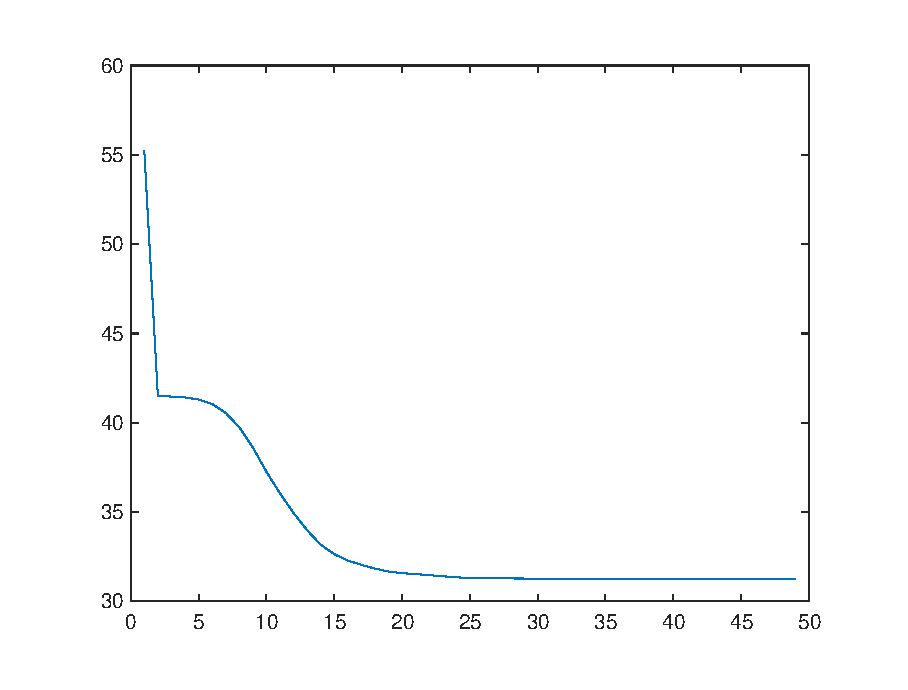
\includegraphics[width=\maxwidth{56.196688409433015em}]{figure_1.eps}
\end{center}

\begin{par}
\begin{flushleft}
Now let's begin the inference system and problem definition
\end{flushleft}
\end{par}

\begin{par}
\begin{flushleft}
We have a 5 inputs 1 output FIs that will be trained using a cascading GA and then for the inference, we will use 2 systems, a TSK 1st order and a TSK 0 order to compare efficiency.
\end{flushleft}
\end{par}

\begin{matlabcode}
% GA parameters
% stochastic rates :
selection_rate=0.01;
elitism_rate=0.001;
mutation_rate=0.3;

% generational parameters
Popsize=200;
maxgen=500;
\end{matlabcode}

\begin{par}
\begin{flushleft}
Let's initialize both the TSKs
\end{flushleft}
\end{par}

\begin{matlabcode}
%TSK0_pop=initTSK0(Popsize);
cluster_pop=initfcm(Popsize,clusters);
% TSK1_pop=initTSK1(Popsize);
% TSK1_pop=TSK1_pop';
%TSK0_pop=TSK0_pop';
parfor i=1:Popsize
    fit0(i)=fitfcm(cluster_pop{i},datatrain,clusters);
end
\end{matlabcode}

\begin{par}
\begin{flushleft}
now let's do the optimization
\end{flushleft}
\end{par}

\begin{matlabcode}
bestfit=[];
for gen=1:maxgen
    
    mutation_rate=max(0.5,1-gen/maxgen);
    [num_elites,pool] = selection(cluster_pop, fit0, selection_rate,Popsize,elitism_rate);
    cluster_pop = reproduction(pool, mutation_rate, Popsize,num_elites,clusters);
    
    % now the new fitness
    bestfit(gen)=min(fit0); % store best fitness
    parfor i=1:Popsize
        newfit(i)=fitfcm(cluster_pop{i},datatrain,clusters);
    end
    fit0=newfit;
    disp(["gen" gen ", best fit = " bestfit(gen) "avg=" bestfit(gen)/length(datatrain)])
end
\end{matlabcode}
\begin{matlaboutput}
    "gen"    "1"    ", best fit = "    "8205.8065"    "avg="    "6.8211"

    "gen"    "2"    ", best fit = "    "8205.8065"    "avg="    "6.8211"

    "gen"    "3"    ", best fit = "    "8143.8061"    "avg="    "6.7696"

    "gen"    "4"    ", best fit = "    "8143.8061"    "avg="    "6.7696"

    "gen"    "5"    ", best fit = "    "8143.8061"    "avg="    "6.7696"

    "gen"    "6"    ", best fit = "    "8143.8061"    "avg="    "6.7696"

    "gen"    "7"    ", best fit = "    "8143.8061"    "avg="    "6.7696"

    "gen"    "8"    ", best fit = "    "8143.8061"    "avg="    "6.7696"

    "gen"    "9"    ", best fit = "    "8143.8061"    "avg="    "6.7696"

    "gen"    "10"    ", best fit = "    "8143.8061"    "avg="    "6.7696"

    "gen"    "11"    ", best fit = "    "7629.8112"    "avg="    "6.3423"

    "gen"    "12"    ", best fit = "    "7629.8112"    "avg="    "6.3423"

    "gen"    "13"    ", best fit = "    "7629.8112"    "avg="    "6.3423"

    "gen"    "14"    ", best fit = "    "6718.7445"    "avg="    "5.585"

    "gen"    "15"    ", best fit = "    "6718.7445"    "avg="    "5.585"

    "gen"    "16"    ", best fit = "    "6718.7445"    "avg="    "5.585"

    "gen"    "17"    ", best fit = "    "6718.7445"    "avg="    "5.585"

    "gen"    "18"    ", best fit = "    "6718.7445"    "avg="    "5.585"

    "gen"    "19"    ", best fit = "    "6718.7445"    "avg="    "5.585"

    "gen"    "20"    ", best fit = "    "6718.7445"    "avg="    "5.585"

    "gen"    "21"    ", best fit = "    "6718.7445"    "avg="    "5.585"

    "gen"    "22"    ", best fit = "    "6718.7445"    "avg="    "5.585"

    "gen"    "23"    ", best fit = "    "6718.7445"    "avg="    "5.585"

    "gen"    "24"    ", best fit = "    "6718.7445"    "avg="    "5.585"

    "gen"    "25"    ", best fit = "    "6718.7445"    "avg="    "5.585"

    "gen"    "26"    ", best fit = "    "6718.7445"    "avg="    "5.585"

    "gen"    "27"    ", best fit = "    "6718.7445"    "avg="    "5.585"

    "gen"    "28"    ", best fit = "    "6718.7445"    "avg="    "5.585"

    "gen"    "29"    ", best fit = "    "6718.7445"    "avg="    "5.585"

    "gen"    "30"    ", best fit = "    "6718.7445"    "avg="    "5.585"

    "gen"    "31"    ", best fit = "    "6718.7445"    "avg="    "5.585"

    "gen"    "32"    ", best fit = "    "6718.7445"    "avg="    "5.585"

    "gen"    "33"    ", best fit = "    "6718.7445"    "avg="    "5.585"

    "gen"    "34"    ", best fit = "    "6718.7445"    "avg="    "5.585"

    "gen"    "35"    ", best fit = "    "6718.7445"    "avg="    "5.585"

    "gen"    "36"    ", best fit = "    "6718.7445"    "avg="    "5.585"

    "gen"    "37"    ", best fit = "    "6718.7445"    "avg="    "5.585"

    "gen"    "38"    ", best fit = "    "6718.7445"    "avg="    "5.585"

    "gen"    "39"    ", best fit = "    "6718.7445"    "avg="    "5.585"

    "gen"    "40"    ", best fit = "    "6718.7445"    "avg="    "5.585"

    "gen"    "41"    ", best fit = "    "6718.7445"    "avg="    "5.585"

    "gen"    "42"    ", best fit = "    "6718.7445"    "avg="    "5.585"

    "gen"    "43"    ", best fit = "    "6718.7445"    "avg="    "5.585"

    "gen"    "44"    ", best fit = "    "6718.7445"    "avg="    "5.585"

    "gen"    "45"    ", best fit = "    "6718.7445"    "avg="    "5.585"

    "gen"    "46"    ", best fit = "    "6718.7445"    "avg="    "5.585"

    "gen"    "47"    ", best fit = "    "6718.7445"    "avg="    "5.585"

    "gen"    "48"    ", best fit = "    "6718.7445"    "avg="    "5.585"

    "gen"    "49"    ", best fit = "    "6718.7445"    "avg="    "5.585"

    "gen"    "50"    ", best fit = "    "6718.7445"    "avg="    "5.585"

    "gen"    "51"    ", best fit = "    "6718.7445"    "avg="    "5.585"

    "gen"    "52"    ", best fit = "    "6718.7445"    "avg="    "5.585"

    "gen"    "53"    ", best fit = "    "6718.7445"    "avg="    "5.585"

    "gen"    "54"    ", best fit = "    "6718.7445"    "avg="    "5.585"

    "gen"    "55"    ", best fit = "    "5906.5591"    "avg="    "4.9099"

    "gen"    "56"    ", best fit = "    "5906.5591"    "avg="    "4.9099"

    "gen"    "57"    ", best fit = "    "5906.5591"    "avg="    "4.9099"

    "gen"    "58"    ", best fit = "    "5906.5591"    "avg="    "4.9099"

    "gen"    "59"    ", best fit = "    "5906.5591"    "avg="    "4.9099"

    "gen"    "60"    ", best fit = "    "5906.5591"    "avg="    "4.9099"

    "gen"    "61"    ", best fit = "    "5906.5591"    "avg="    "4.9099"

    "gen"    "62"    ", best fit = "    "5906.5591"    "avg="    "4.9099"

    "gen"    "63"    ", best fit = "    "5906.5591"    "avg="    "4.9099"

    "gen"    "64"    ", best fit = "    "5906.5591"    "avg="    "4.9099"

    "gen"    "65"    ", best fit = "    "5906.5591"    "avg="    "4.9099"

    "gen"    "66"    ", best fit = "    "5906.5591"    "avg="    "4.9099"

    "gen"    "67"    ", best fit = "    "5906.5591"    "avg="    "4.9099"

    "gen"    "68"    ", best fit = "    "5906.5591"    "avg="    "4.9099"

    "gen"    "69"    ", best fit = "    "5906.5591"    "avg="    "4.9099"

    "gen"    "70"    ", best fit = "    "5906.5591"    "avg="    "4.9099"

    "gen"    "71"    ", best fit = "    "5906.5591"    "avg="    "4.9099"

    "gen"    "72"    ", best fit = "    "5896.1843"    "avg="    "4.9012"

    "gen"    "73"    ", best fit = "    "5896.1843"    "avg="    "4.9012"

    "gen"    "74"    ", best fit = "    "5896.1843"    "avg="    "4.9012"

    "gen"    "75"    ", best fit = "    "5896.1843"    "avg="    "4.9012"

    "gen"    "76"    ", best fit = "    "5896.1843"    "avg="    "4.9012"

    "gen"    "77"    ", best fit = "    "5896.1843"    "avg="    "4.9012"

    "gen"    "78"    ", best fit = "    "5896.1843"    "avg="    "4.9012"

    "gen"    "79"    ", best fit = "    "5896.1843"    "avg="    "4.9012"

    "gen"    "80"    ", best fit = "    "5896.1843"    "avg="    "4.9012"

    "gen"    "81"    ", best fit = "    "5896.1843"    "avg="    "4.9012"

    "gen"    "82"    ", best fit = "    "5896.1843"    "avg="    "4.9012"

    "gen"    "83"    ", best fit = "    "5896.1843"    "avg="    "4.9012"

    "gen"    "84"    ", best fit = "    "5896.1843"    "avg="    "4.9012"

    "gen"    "85"    ", best fit = "    "5894.3782"    "avg="    "4.8997"

    "gen"    "86"    ", best fit = "    "5894.3782"    "avg="    "4.8997"

    "gen"    "87"    ", best fit = "    "5894.3782"    "avg="    "4.8997"

    "gen"    "88"    ", best fit = "    "5894.3782"    "avg="    "4.8997"

    "gen"    "89"    ", best fit = "    "5894.3782"    "avg="    "4.8997"

    "gen"    "90"    ", best fit = "    "5894.3782"    "avg="    "4.8997"

    "gen"    "91"    ", best fit = "    "5894.3782"    "avg="    "4.8997"

    "gen"    "92"    ", best fit = "    "5894.3782"    "avg="    "4.8997"

    "gen"    "93"    ", best fit = "    "5894.3782"    "avg="    "4.8997"

    "gen"    "94"    ", best fit = "    "5894.3782"    "avg="    "4.8997"

    "gen"    "95"    ", best fit = "    "5894.3782"    "avg="    "4.8997"

    "gen"    "96"    ", best fit = "    "5894.3782"    "avg="    "4.8997"

    "gen"    "97"    ", best fit = "    "5894.3782"    "avg="    "4.8997"

    "gen"    "98"    ", best fit = "    "5894.3782"    "avg="    "4.8997"

    "gen"    "99"    ", best fit = "    "5894.3782"    "avg="    "4.8997"

    "gen"    "100"    ", best fit = "    "5894.3782"    "avg="    "4.8997"

    "gen"    "101"    ", best fit = "    "5894.3782"    "avg="    "4.8997"

    "gen"    "102"    ", best fit = "    "5894.3782"    "avg="    "4.8997"

    "gen"    "103"    ", best fit = "    "5894.3782"    "avg="    "4.8997"

    "gen"    "104"    ", best fit = "    "5894.3782"    "avg="    "4.8997"

    "gen"    "105"    ", best fit = "    "5894.3782"    "avg="    "4.8997"

    "gen"    "106"    ", best fit = "    "5894.3782"    "avg="    "4.8997"

    "gen"    "107"    ", best fit = "    "5894.3782"    "avg="    "4.8997"

    "gen"    "108"    ", best fit = "    "5894.3782"    "avg="    "4.8997"

    "gen"    "109"    ", best fit = "    "5894.3782"    "avg="    "4.8997"

    "gen"    "110"    ", best fit = "    "5894.3782"    "avg="    "4.8997"

    "gen"    "111"    ", best fit = "    "5894.3782"    "avg="    "4.8997"

    "gen"    "112"    ", best fit = "    "5894.3782"    "avg="    "4.8997"

    "gen"    "113"    ", best fit = "    "5894.3782"    "avg="    "4.8997"

    "gen"    "114"    ", best fit = "    "5894.3782"    "avg="    "4.8997"

    "gen"    "115"    ", best fit = "    "5894.3782"    "avg="    "4.8997"

    "gen"    "116"    ", best fit = "    "5894.3782"    "avg="    "4.8997"

    "gen"    "117"    ", best fit = "    "5894.3782"    "avg="    "4.8997"

    "gen"    "118"    ", best fit = "    "5894.3782"    "avg="    "4.8997"

    "gen"    "119"    ", best fit = "    "5894.3782"    "avg="    "4.8997"

    "gen"    "120"    ", best fit = "    "5894.3782"    "avg="    "4.8997"

    "gen"    "121"    ", best fit = "    "5894.3782"    "avg="    "4.8997"

    "gen"    "122"    ", best fit = "    "5894.3782"    "avg="    "4.8997"

    "gen"    "123"    ", best fit = "    "5894.3782"    "avg="    "4.8997"

    "gen"    "124"    ", best fit = "    "5894.3782"    "avg="    "4.8997"

    "gen"    "125"    ", best fit = "    "5894.3782"    "avg="    "4.8997"

    "gen"    "126"    ", best fit = "    "5894.3782"    "avg="    "4.8997"

    "gen"    "127"    ", best fit = "    "5894.3782"    "avg="    "4.8997"

    "gen"    "128"    ", best fit = "    "5894.3782"    "avg="    "4.8997"

    "gen"    "129"    ", best fit = "    "5894.3782"    "avg="    "4.8997"

    "gen"    "130"    ", best fit = "    "5894.3782"    "avg="    "4.8997"

    "gen"    "131"    ", best fit = "    "5894.3782"    "avg="    "4.8997"

    "gen"    "132"    ", best fit = "    "5894.3782"    "avg="    "4.8997"

    "gen"    "133"    ", best fit = "    "5894.3782"    "avg="    "4.8997"

    "gen"    "134"    ", best fit = "    "5894.3782"    "avg="    "4.8997"

    "gen"    "135"    ", best fit = "    "5894.3782"    "avg="    "4.8997"

    "gen"    "136"    ", best fit = "    "5894.3782"    "avg="    "4.8997"

    "gen"    "137"    ", best fit = "    "5894.3782"    "avg="    "4.8997"

    "gen"    "138"    ", best fit = "    "5894.3782"    "avg="    "4.8997"

    "gen"    "139"    ", best fit = "    "5894.3782"    "avg="    "4.8997"

    "gen"    "140"    ", best fit = "    "5894.3782"    "avg="    "4.8997"

    "gen"    "141"    ", best fit = "    "5894.3782"    "avg="    "4.8997"

    "gen"    "142"    ", best fit = "    "5894.3782"    "avg="    "4.8997"

    "gen"    "143"    ", best fit = "    "5894.3782"    "avg="    "4.8997"

    "gen"    "144"    ", best fit = "    "5894.3782"    "avg="    "4.8997"

    "gen"    "145"    ", best fit = "    "5894.3782"    "avg="    "4.8997"

    "gen"    "146"    ", best fit = "    "5894.3782"    "avg="    "4.8997"

    "gen"    "147"    ", best fit = "    "5894.3782"    "avg="    "4.8997"

    "gen"    "148"    ", best fit = "    "5894.3782"    "avg="    "4.8997"

    "gen"    "149"    ", best fit = "    "5894.3782"    "avg="    "4.8997"

    "gen"    "150"    ", best fit = "    "5894.3782"    "avg="    "4.8997"

    "gen"    "151"    ", best fit = "    "5894.3782"    "avg="    "4.8997"

    "gen"    "152"    ", best fit = "    "5894.3782"    "avg="    "4.8997"

    "gen"    "153"    ", best fit = "    "5894.3782"    "avg="    "4.8997"

    "gen"    "154"    ", best fit = "    "5894.3782"    "avg="    "4.8997"

    "gen"    "155"    ", best fit = "    "5894.3782"    "avg="    "4.8997"

    "gen"    "156"    ", best fit = "    "5894.3782"    "avg="    "4.8997"

    "gen"    "157"    ", best fit = "    "5894.3782"    "avg="    "4.8997"

    "gen"    "158"    ", best fit = "    "5894.3782"    "avg="    "4.8997"

    "gen"    "159"    ", best fit = "    "5894.3782"    "avg="    "4.8997"

    "gen"    "160"    ", best fit = "    "5894.3782"    "avg="    "4.8997"

    "gen"    "161"    ", best fit = "    "5894.3782"    "avg="    "4.8997"

    "gen"    "162"    ", best fit = "    "5894.3782"    "avg="    "4.8997"

    "gen"    "163"    ", best fit = "    "5894.3782"    "avg="    "4.8997"

    "gen"    "164"    ", best fit = "    "5894.3782"    "avg="    "4.8997"

    "gen"    "165"    ", best fit = "    "5894.3782"    "avg="    "4.8997"

    "gen"    "166"    ", best fit = "    "5894.3782"    "avg="    "4.8997"

    "gen"    "167"    ", best fit = "    "5894.3782"    "avg="    "4.8997"

    "gen"    "168"    ", best fit = "    "5894.3782"    "avg="    "4.8997"

    "gen"    "169"    ", best fit = "    "5894.3782"    "avg="    "4.8997"

    "gen"    "170"    ", best fit = "    "5894.3782"    "avg="    "4.8997"

    "gen"    "171"    ", best fit = "    "5894.3782"    "avg="    "4.8997"

    "gen"    "172"    ", best fit = "    "5894.3782"    "avg="    "4.8997"

    "gen"    "173"    ", best fit = "    "5894.3782"    "avg="    "4.8997"

    "gen"    "174"    ", best fit = "    "5894.3782"    "avg="    "4.8997"

    "gen"    "175"    ", best fit = "    "5894.3782"    "avg="    "4.8997"

    "gen"    "176"    ", best fit = "    "5894.3782"    "avg="    "4.8997"

    "gen"    "177"    ", best fit = "    "5894.3782"    "avg="    "4.8997"

    "gen"    "178"    ", best fit = "    "5894.3782"    "avg="    "4.8997"

    "gen"    "179"    ", best fit = "    "5894.3782"    "avg="    "4.8997"

    "gen"    "180"    ", best fit = "    "5894.3782"    "avg="    "4.8997"

    "gen"    "181"    ", best fit = "    "5894.3782"    "avg="    "4.8997"

    "gen"    "182"    ", best fit = "    "5894.3782"    "avg="    "4.8997"

    "gen"    "183"    ", best fit = "    "5894.3782"    "avg="    "4.8997"

    "gen"    "184"    ", best fit = "    "5894.3782"    "avg="    "4.8997"

    "gen"    "185"    ", best fit = "    "5894.3782"    "avg="    "4.8997"

    "gen"    "186"    ", best fit = "    "5894.3782"    "avg="    "4.8997"

    "gen"    "187"    ", best fit = "    "5894.3782"    "avg="    "4.8997"

    "gen"    "188"    ", best fit = "    "5894.3782"    "avg="    "4.8997"

    "gen"    "189"    ", best fit = "    "5894.3782"    "avg="    "4.8997"

    "gen"    "190"    ", best fit = "    "5894.3782"    "avg="    "4.8997"

    "gen"    "191"    ", best fit = "    "5894.3782"    "avg="    "4.8997"

    "gen"    "192"    ", best fit = "    "5894.3782"    "avg="    "4.8997"

    "gen"    "193"    ", best fit = "    "5894.3782"    "avg="    "4.8997"

    "gen"    "194"    ", best fit = "    "5894.3782"    "avg="    "4.8997"

    "gen"    "195"    ", best fit = "    "5894.3782"    "avg="    "4.8997"

    "gen"    "196"    ", best fit = "    "5894.3782"    "avg="    "4.8997"

    "gen"    "197"    ", best fit = "    "5894.3782"    "avg="    "4.8997"

    "gen"    "198"    ", best fit = "    "5894.3782"    "avg="    "4.8997"

    "gen"    "199"    ", best fit = "    "5894.3782"    "avg="    "4.8997"

    "gen"    "200"    ", best fit = "    "5894.3782"    "avg="    "4.8997"

    "gen"    "201"    ", best fit = "    "5894.3782"    "avg="    "4.8997"

    "gen"    "202"    ", best fit = "    "5894.3782"    "avg="    "4.8997"

    "gen"    "203"    ", best fit = "    "5894.3782"    "avg="    "4.8997"

    "gen"    "204"    ", best fit = "    "5894.3782"    "avg="    "4.8997"

    "gen"    "205"    ", best fit = "    "5894.3782"    "avg="    "4.8997"

    "gen"    "206"    ", best fit = "    "5894.3782"    "avg="    "4.8997"

    "gen"    "207"    ", best fit = "    "5894.3782"    "avg="    "4.8997"

    "gen"    "208"    ", best fit = "    "5894.3782"    "avg="    "4.8997"

    "gen"    "209"    ", best fit = "    "5894.3782"    "avg="    "4.8997"

    "gen"    "210"    ", best fit = "    "5894.3782"    "avg="    "4.8997"

    "gen"    "211"    ", best fit = "    "5894.3782"    "avg="    "4.8997"

    "gen"    "212"    ", best fit = "    "5894.3782"    "avg="    "4.8997"

    "gen"    "213"    ", best fit = "    "5894.3782"    "avg="    "4.8997"

    "gen"    "214"    ", best fit = "    "5894.3782"    "avg="    "4.8997"

    "gen"    "215"    ", best fit = "    "5894.3782"    "avg="    "4.8997"

    "gen"    "216"    ", best fit = "    "5894.3782"    "avg="    "4.8997"

    "gen"    "217"    ", best fit = "    "5894.3782"    "avg="    "4.8997"

    "gen"    "218"    ", best fit = "    "5894.3782"    "avg="    "4.8997"

    "gen"    "219"    ", best fit = "    "5894.3782"    "avg="    "4.8997"

    "gen"    "220"    ", best fit = "    "5894.3782"    "avg="    "4.8997"

    "gen"    "221"    ", best fit = "    "5894.3782"    "avg="    "4.8997"

    "gen"    "222"    ", best fit = "    "5894.3782"    "avg="    "4.8997"

    "gen"    "223"    ", best fit = "    "5894.3782"    "avg="    "4.8997"

    "gen"    "224"    ", best fit = "    "5894.3782"    "avg="    "4.8997"

    "gen"    "225"    ", best fit = "    "5894.3782"    "avg="    "4.8997"

    "gen"    "226"    ", best fit = "    "5894.3782"    "avg="    "4.8997"

    "gen"    "227"    ", best fit = "    "5894.3782"    "avg="    "4.8997"

    "gen"    "228"    ", best fit = "    "5894.3782"    "avg="    "4.8997"

    "gen"    "229"    ", best fit = "    "5894.3782"    "avg="    "4.8997"

    "gen"    "230"    ", best fit = "    "5894.3782"    "avg="    "4.8997"

    "gen"    "231"    ", best fit = "    "5894.3782"    "avg="    "4.8997"

    "gen"    "232"    ", best fit = "    "5894.3782"    "avg="    "4.8997"

    "gen"    "233"    ", best fit = "    "5894.3782"    "avg="    "4.8997"

    "gen"    "234"    ", best fit = "    "5894.3782"    "avg="    "4.8997"

    "gen"    "235"    ", best fit = "    "5894.3782"    "avg="    "4.8997"

    "gen"    "236"    ", best fit = "    "5894.3782"    "avg="    "4.8997"

    "gen"    "237"    ", best fit = "    "5894.3782"    "avg="    "4.8997"

    "gen"    "238"    ", best fit = "    "5894.3782"    "avg="    "4.8997"

    "gen"    "239"    ", best fit = "    "5894.3782"    "avg="    "4.8997"

    "gen"    "240"    ", best fit = "    "5894.3782"    "avg="    "4.8997"

    "gen"    "241"    ", best fit = "    "5894.3782"    "avg="    "4.8997"

    "gen"    "242"    ", best fit = "    "5894.3782"    "avg="    "4.8997"

    "gen"    "243"    ", best fit = "    "5894.3782"    "avg="    "4.8997"

    "gen"    "244"    ", best fit = "    "5894.3782"    "avg="    "4.8997"

    "gen"    "245"    ", best fit = "    "5894.3782"    "avg="    "4.8997"

    "gen"    "246"    ", best fit = "    "5894.3782"    "avg="    "4.8997"

    "gen"    "247"    ", best fit = "    "5894.3782"    "avg="    "4.8997"

    "gen"    "248"    ", best fit = "    "5894.3782"    "avg="    "4.8997"

    "gen"    "249"    ", best fit = "    "5894.3782"    "avg="    "4.8997"

    "gen"    "250"    ", best fit = "    "5894.3782"    "avg="    "4.8997"

    "gen"    "251"    ", best fit = "    "5894.3782"    "avg="    "4.8997"

    "gen"    "252"    ", best fit = "    "5894.3782"    "avg="    "4.8997"

    "gen"    "253"    ", best fit = "    "5894.3782"    "avg="    "4.8997"

    "gen"    "254"    ", best fit = "    "5894.3782"    "avg="    "4.8997"

    "gen"    "255"    ", best fit = "    "5894.3782"    "avg="    "4.8997"

    "gen"    "256"    ", best fit = "    "5894.3782"    "avg="    "4.8997"

    "gen"    "257"    ", best fit = "    "5894.3782"    "avg="    "4.8997"

    "gen"    "258"    ", best fit = "    "5894.3782"    "avg="    "4.8997"

    "gen"    "259"    ", best fit = "    "5894.3782"    "avg="    "4.8997"

    "gen"    "260"    ", best fit = "    "5894.3782"    "avg="    "4.8997"

    "gen"    "261"    ", best fit = "    "5894.3782"    "avg="    "4.8997"

    "gen"    "262"    ", best fit = "    "5894.3782"    "avg="    "4.8997"

    "gen"    "263"    ", best fit = "    "5894.3782"    "avg="    "4.8997"

    "gen"    "264"    ", best fit = "    "5894.3782"    "avg="    "4.8997"

    "gen"    "265"    ", best fit = "    "5894.3782"    "avg="    "4.8997"

    "gen"    "266"    ", best fit = "    "5894.3782"    "avg="    "4.8997"

    "gen"    "267"    ", best fit = "    "5894.3782"    "avg="    "4.8997"

    "gen"    "268"    ", best fit = "    "5894.3782"    "avg="    "4.8997"

    "gen"    "269"    ", best fit = "    "5894.3782"    "avg="    "4.8997"

    "gen"    "270"    ", best fit = "    "5894.3782"    "avg="    "4.8997"

    "gen"    "271"    ", best fit = "    "5894.3782"    "avg="    "4.8997"

    "gen"    "272"    ", best fit = "    "5894.3782"    "avg="    "4.8997"

    "gen"    "273"    ", best fit = "    "5894.3782"    "avg="    "4.8997"

    "gen"    "274"    ", best fit = "    "5894.3782"    "avg="    "4.8997"

    "gen"    "275"    ", best fit = "    "5894.3782"    "avg="    "4.8997"

    "gen"    "276"    ", best fit = "    "5894.3782"    "avg="    "4.8997"

    "gen"    "277"    ", best fit = "    "5894.3782"    "avg="    "4.8997"

    "gen"    "278"    ", best fit = "    "5894.3782"    "avg="    "4.8997"

    "gen"    "279"    ", best fit = "    "5894.3782"    "avg="    "4.8997"

    "gen"    "280"    ", best fit = "    "5894.3782"    "avg="    "4.8997"

    "gen"    "281"    ", best fit = "    "5894.3782"    "avg="    "4.8997"

    "gen"    "282"    ", best fit = "    "5894.3782"    "avg="    "4.8997"

    "gen"    "283"    ", best fit = "    "5894.3782"    "avg="    "4.8997"

    "gen"    "284"    ", best fit = "    "5894.3782"    "avg="    "4.8997"

    "gen"    "285"    ", best fit = "    "5894.3782"    "avg="    "4.8997"

    "gen"    "286"    ", best fit = "    "5894.3782"    "avg="    "4.8997"

    "gen"    "287"    ", best fit = "    "5894.3782"    "avg="    "4.8997"

    "gen"    "288"    ", best fit = "    "5894.3782"    "avg="    "4.8997"

    "gen"    "289"    ", best fit = "    "5894.3782"    "avg="    "4.8997"

    "gen"    "290"    ", best fit = "    "5894.3782"    "avg="    "4.8997"

    "gen"    "291"    ", best fit = "    "5894.3782"    "avg="    "4.8997"

    "gen"    "292"    ", best fit = "    "5894.3782"    "avg="    "4.8997"

    "gen"    "293"    ", best fit = "    "5894.3782"    "avg="    "4.8997"

    "gen"    "294"    ", best fit = "    "5894.3782"    "avg="    "4.8997"

    "gen"    "295"    ", best fit = "    "5894.3782"    "avg="    "4.8997"

    "gen"    "296"    ", best fit = "    "5894.3782"    "avg="    "4.8997"

    "gen"    "297"    ", best fit = "    "5894.3782"    "avg="    "4.8997"

    "gen"    "298"    ", best fit = "    "5894.3782"    "avg="    "4.8997"

    "gen"    "299"    ", best fit = "    "5894.3782"    "avg="    "4.8997"

    "gen"    "300"    ", best fit = "    "5894.3782"    "avg="    "4.8997"

    "gen"    "301"    ", best fit = "    "5894.3782"    "avg="    "4.8997"

    "gen"    "302"    ", best fit = "    "5894.3782"    "avg="    "4.8997"

    "gen"    "303"    ", best fit = "    "5894.3782"    "avg="    "4.8997"

    "gen"    "304"    ", best fit = "    "5894.3782"    "avg="    "4.8997"

    "gen"    "305"    ", best fit = "    "5894.3782"    "avg="    "4.8997"

    "gen"    "306"    ", best fit = "    "5894.3782"    "avg="    "4.8997"

    "gen"    "307"    ", best fit = "    "5894.3782"    "avg="    "4.8997"

    "gen"    "308"    ", best fit = "    "5894.3782"    "avg="    "4.8997"

    "gen"    "309"    ", best fit = "    "5894.3782"    "avg="    "4.8997"

    "gen"    "310"    ", best fit = "    "5894.3782"    "avg="    "4.8997"

    "gen"    "311"    ", best fit = "    "5894.3782"    "avg="    "4.8997"

    "gen"    "312"    ", best fit = "    "5894.3782"    "avg="    "4.8997"

    "gen"    "313"    ", best fit = "    "5894.3782"    "avg="    "4.8997"

    "gen"    "314"    ", best fit = "    "5894.3782"    "avg="    "4.8997"

    "gen"    "315"    ", best fit = "    "5894.3782"    "avg="    "4.8997"

    "gen"    "316"    ", best fit = "    "5894.3782"    "avg="    "4.8997"

    "gen"    "317"    ", best fit = "    "5894.3782"    "avg="    "4.8997"

    "gen"    "318"    ", best fit = "    "5894.3782"    "avg="    "4.8997"

    "gen"    "319"    ", best fit = "    "5894.3782"    "avg="    "4.8997"

    "gen"    "320"    ", best fit = "    "5894.3782"    "avg="    "4.8997"

    "gen"    "321"    ", best fit = "    "5894.3782"    "avg="    "4.8997"

    "gen"    "322"    ", best fit = "    "5894.3782"    "avg="    "4.8997"

    "gen"    "323"    ", best fit = "    "5894.3782"    "avg="    "4.8997"

    "gen"    "324"    ", best fit = "    "5894.3782"    "avg="    "4.8997"

    "gen"    "325"    ", best fit = "    "5894.3782"    "avg="    "4.8997"

    "gen"    "326"    ", best fit = "    "5894.3782"    "avg="    "4.8997"

    "gen"    "327"    ", best fit = "    "5894.3782"    "avg="    "4.8997"

    "gen"    "328"    ", best fit = "    "5894.3782"    "avg="    "4.8997"

    "gen"    "329"    ", best fit = "    "5894.3782"    "avg="    "4.8997"

    "gen"    "330"    ", best fit = "    "5894.3782"    "avg="    "4.8997"

    "gen"    "331"    ", best fit = "    "5894.3782"    "avg="    "4.8997"

    "gen"    "332"    ", best fit = "    "5894.3782"    "avg="    "4.8997"

    "gen"    "333"    ", best fit = "    "5894.3782"    "avg="    "4.8997"

    "gen"    "334"    ", best fit = "    "5894.3782"    "avg="    "4.8997"

    "gen"    "335"    ", best fit = "    "5894.3782"    "avg="    "4.8997"

    "gen"    "336"    ", best fit = "    "5894.3782"    "avg="    "4.8997"

    "gen"    "337"    ", best fit = "    "5894.3782"    "avg="    "4.8997"

    "gen"    "338"    ", best fit = "    "5894.3782"    "avg="    "4.8997"

    "gen"    "339"    ", best fit = "    "5894.3782"    "avg="    "4.8997"

    "gen"    "340"    ", best fit = "    "5894.3782"    "avg="    "4.8997"

    "gen"    "341"    ", best fit = "    "5894.3782"    "avg="    "4.8997"

    "gen"    "342"    ", best fit = "    "5894.3782"    "avg="    "4.8997"

    "gen"    "343"    ", best fit = "    "5894.3782"    "avg="    "4.8997"

    "gen"    "344"    ", best fit = "    "5894.3782"    "avg="    "4.8997"

    "gen"    "345"    ", best fit = "    "5894.3782"    "avg="    "4.8997"

    "gen"    "346"    ", best fit = "    "5894.3782"    "avg="    "4.8997"

    "gen"    "347"    ", best fit = "    "5894.3782"    "avg="    "4.8997"

    "gen"    "348"    ", best fit = "    "5894.3782"    "avg="    "4.8997"

    "gen"    "349"    ", best fit = "    "5894.3782"    "avg="    "4.8997"

    "gen"    "350"    ", best fit = "    "5894.3782"    "avg="    "4.8997"

    "gen"    "351"    ", best fit = "    "5894.3782"    "avg="    "4.8997"

    "gen"    "352"    ", best fit = "    "5894.3782"    "avg="    "4.8997"

    "gen"    "353"    ", best fit = "    "5894.3782"    "avg="    "4.8997"

    "gen"    "354"    ", best fit = "    "5894.3782"    "avg="    "4.8997"

    "gen"    "355"    ", best fit = "    "5894.3782"    "avg="    "4.8997"

    "gen"    "356"    ", best fit = "    "5894.3782"    "avg="    "4.8997"

    "gen"    "357"    ", best fit = "    "5894.3782"    "avg="    "4.8997"

    "gen"    "358"    ", best fit = "    "5894.3782"    "avg="    "4.8997"

    "gen"    "359"    ", best fit = "    "5894.3782"    "avg="    "4.8997"

    "gen"    "360"    ", best fit = "    "5894.3782"    "avg="    "4.8997"

    "gen"    "361"    ", best fit = "    "5894.3782"    "avg="    "4.8997"

    "gen"    "362"    ", best fit = "    "5894.3782"    "avg="    "4.8997"

    "gen"    "363"    ", best fit = "    "5894.3782"    "avg="    "4.8997"

    "gen"    "364"    ", best fit = "    "5894.3782"    "avg="    "4.8997"

    "gen"    "365"    ", best fit = "    "5894.3782"    "avg="    "4.8997"

    "gen"    "366"    ", best fit = "    "5894.3782"    "avg="    "4.8997"

    "gen"    "367"    ", best fit = "    "5894.3782"    "avg="    "4.8997"

    "gen"    "368"    ", best fit = "    "5894.3782"    "avg="    "4.8997"

    "gen"    "369"    ", best fit = "    "5894.3782"    "avg="    "4.8997"

    "gen"    "370"    ", best fit = "    "5894.3782"    "avg="    "4.8997"

    "gen"    "371"    ", best fit = "    "5894.3782"    "avg="    "4.8997"

    "gen"    "372"    ", best fit = "    "5894.3782"    "avg="    "4.8997"

    "gen"    "373"    ", best fit = "    "5894.3782"    "avg="    "4.8997"

    "gen"    "374"    ", best fit = "    "5894.3782"    "avg="    "4.8997"

    "gen"    "375"    ", best fit = "    "5894.3782"    "avg="    "4.8997"

    "gen"    "376"    ", best fit = "    "5894.3782"    "avg="    "4.8997"

    "gen"    "377"    ", best fit = "    "5894.3782"    "avg="    "4.8997"

    "gen"    "378"    ", best fit = "    "5894.3782"    "avg="    "4.8997"

    "gen"    "379"    ", best fit = "    "5894.3782"    "avg="    "4.8997"

    "gen"    "380"    ", best fit = "    "5894.3782"    "avg="    "4.8997"

    "gen"    "381"    ", best fit = "    "5894.3782"    "avg="    "4.8997"

    "gen"    "382"    ", best fit = "    "5894.3782"    "avg="    "4.8997"

    "gen"    "383"    ", best fit = "    "5894.3782"    "avg="    "4.8997"

    "gen"    "384"    ", best fit = "    "5894.3782"    "avg="    "4.8997"

    "gen"    "385"    ", best fit = "    "5894.3782"    "avg="    "4.8997"

    "gen"    "386"    ", best fit = "    "5894.3782"    "avg="    "4.8997"

    "gen"    "387"    ", best fit = "    "5894.3782"    "avg="    "4.8997"

    "gen"    "388"    ", best fit = "    "5894.3782"    "avg="    "4.8997"

    "gen"    "389"    ", best fit = "    "5894.3782"    "avg="    "4.8997"

    "gen"    "390"    ", best fit = "    "5894.3782"    "avg="    "4.8997"

    "gen"    "391"    ", best fit = "    "5894.3782"    "avg="    "4.8997"

    "gen"    "392"    ", best fit = "    "5894.3782"    "avg="    "4.8997"

    "gen"    "393"    ", best fit = "    "5894.3782"    "avg="    "4.8997"

    "gen"    "394"    ", best fit = "    "5894.3782"    "avg="    "4.8997"

    "gen"    "395"    ", best fit = "    "5871.5683"    "avg="    "4.8808"

    "gen"    "396"    ", best fit = "    "5871.5683"    "avg="    "4.8808"

    "gen"    "397"    ", best fit = "    "5871.5683"    "avg="    "4.8808"

    "gen"    "398"    ", best fit = "    "5871.5683"    "avg="    "4.8808"

    "gen"    "399"    ", best fit = "    "5871.5683"    "avg="    "4.8808"

    "gen"    "400"    ", best fit = "    "5871.5683"    "avg="    "4.8808"

    "gen"    "401"    ", best fit = "    "5871.5683"    "avg="    "4.8808"

    "gen"    "402"    ", best fit = "    "5871.5683"    "avg="    "4.8808"

    "gen"    "403"    ", best fit = "    "5871.5683"    "avg="    "4.8808"

    "gen"    "404"    ", best fit = "    "5871.5683"    "avg="    "4.8808"

    "gen"    "405"    ", best fit = "    "5871.5683"    "avg="    "4.8808"

    "gen"    "406"    ", best fit = "    "5871.5683"    "avg="    "4.8808"

    "gen"    "407"    ", best fit = "    "5871.5683"    "avg="    "4.8808"

    "gen"    "408"    ", best fit = "    "5871.5683"    "avg="    "4.8808"

    "gen"    "409"    ", best fit = "    "5871.5683"    "avg="    "4.8808"

    "gen"    "410"    ", best fit = "    "5871.5683"    "avg="    "4.8808"

    "gen"    "411"    ", best fit = "    "5871.5683"    "avg="    "4.8808"

    "gen"    "412"    ", best fit = "    "5871.5683"    "avg="    "4.8808"

    "gen"    "413"    ", best fit = "    "5871.5683"    "avg="    "4.8808"

    "gen"    "414"    ", best fit = "    "5871.5683"    "avg="    "4.8808"

    "gen"    "415"    ", best fit = "    "5871.5683"    "avg="    "4.8808"

    "gen"    "416"    ", best fit = "    "5871.5683"    "avg="    "4.8808"

    "gen"    "417"    ", best fit = "    "5871.5683"    "avg="    "4.8808"

    "gen"    "418"    ", best fit = "    "5871.5683"    "avg="    "4.8808"

    "gen"    "419"    ", best fit = "    "5871.5683"    "avg="    "4.8808"

    "gen"    "420"    ", best fit = "    "5871.5683"    "avg="    "4.8808"

    "gen"    "421"    ", best fit = "    "5871.5683"    "avg="    "4.8808"

    "gen"    "422"    ", best fit = "    "5871.5683"    "avg="    "4.8808"

    "gen"    "423"    ", best fit = "    "5871.5683"    "avg="    "4.8808"

    "gen"    "424"    ", best fit = "    "5871.5683"    "avg="    "4.8808"

    "gen"    "425"    ", best fit = "    "5871.5683"    "avg="    "4.8808"

    "gen"    "426"    ", best fit = "    "5871.5683"    "avg="    "4.8808"

    "gen"    "427"    ", best fit = "    "5871.5683"    "avg="    "4.8808"

    "gen"    "428"    ", best fit = "    "5871.5683"    "avg="    "4.8808"

    "gen"    "429"    ", best fit = "    "5871.5683"    "avg="    "4.8808"

    "gen"    "430"    ", best fit = "    "5871.5683"    "avg="    "4.8808"

    "gen"    "431"    ", best fit = "    "5871.5683"    "avg="    "4.8808"

    "gen"    "432"    ", best fit = "    "5871.5683"    "avg="    "4.8808"

    "gen"    "433"    ", best fit = "    "5871.5683"    "avg="    "4.8808"

    "gen"    "434"    ", best fit = "    "5871.5683"    "avg="    "4.8808"

    "gen"    "435"    ", best fit = "    "5871.5683"    "avg="    "4.8808"

    "gen"    "436"    ", best fit = "    "5871.5683"    "avg="    "4.8808"

    "gen"    "437"    ", best fit = "    "5871.5683"    "avg="    "4.8808"

    "gen"    "438"    ", best fit = "    "5871.5683"    "avg="    "4.8808"

    "gen"    "439"    ", best fit = "    "5871.5683"    "avg="    "4.8808"

    "gen"    "440"    ", best fit = "    "5871.5683"    "avg="    "4.8808"

    "gen"    "441"    ", best fit = "    "5871.5683"    "avg="    "4.8808"

    "gen"    "442"    ", best fit = "    "5871.5683"    "avg="    "4.8808"

    "gen"    "443"    ", best fit = "    "5871.5683"    "avg="    "4.8808"

    "gen"    "444"    ", best fit = "    "5871.5683"    "avg="    "4.8808"

    "gen"    "445"    ", best fit = "    "5871.5683"    "avg="    "4.8808"

    "gen"    "446"    ", best fit = "    "5871.5683"    "avg="    "4.8808"

    "gen"    "447"    ", best fit = "    "5871.5683"    "avg="    "4.8808"

    "gen"    "448"    ", best fit = "    "5871.5683"    "avg="    "4.8808"

    "gen"    "449"    ", best fit = "    "5871.5683"    "avg="    "4.8808"

    "gen"    "450"    ", best fit = "    "5871.5683"    "avg="    "4.8808"

    "gen"    "451"    ", best fit = "    "5871.5683"    "avg="    "4.8808"

    "gen"    "452"    ", best fit = "    "5871.5683"    "avg="    "4.8808"

    "gen"    "453"    ", best fit = "    "5871.5683"    "avg="    "4.8808"

    "gen"    "454"    ", best fit = "    "5871.5683"    "avg="    "4.8808"

    "gen"    "455"    ", best fit = "    "5871.5683"    "avg="    "4.8808"

    "gen"    "456"    ", best fit = "    "5871.5683"    "avg="    "4.8808"

    "gen"    "457"    ", best fit = "    "5871.5683"    "avg="    "4.8808"

    "gen"    "458"    ", best fit = "    "5871.5683"    "avg="    "4.8808"

    "gen"    "459"    ", best fit = "    "5871.5683"    "avg="    "4.8808"

    "gen"    "460"    ", best fit = "    "5871.5683"    "avg="    "4.8808"

    "gen"    "461"    ", best fit = "    "5871.5683"    "avg="    "4.8808"

    "gen"    "462"    ", best fit = "    "5871.5683"    "avg="    "4.8808"

    "gen"    "463"    ", best fit = "    "5871.5683"    "avg="    "4.8808"

    "gen"    "464"    ", best fit = "    "5871.5683"    "avg="    "4.8808"

    "gen"    "465"    ", best fit = "    "5871.5683"    "avg="    "4.8808"

    "gen"    "466"    ", best fit = "    "5871.5683"    "avg="    "4.8808"

    "gen"    "467"    ", best fit = "    "5871.5683"    "avg="    "4.8808"

    "gen"    "468"    ", best fit = "    "5871.5683"    "avg="    "4.8808"

    "gen"    "469"    ", best fit = "    "5871.5683"    "avg="    "4.8808"

    "gen"    "470"    ", best fit = "    "5871.5683"    "avg="    "4.8808"

    "gen"    "471"    ", best fit = "    "5871.5683"    "avg="    "4.8808"

    "gen"    "472"    ", best fit = "    "5871.5683"    "avg="    "4.8808"

    "gen"    "473"    ", best fit = "    "5871.5683"    "avg="    "4.8808"

    "gen"    "474"    ", best fit = "    "5871.5683"    "avg="    "4.8808"

    "gen"    "475"    ", best fit = "    "5871.5683"    "avg="    "4.8808"

    "gen"    "476"    ", best fit = "    "5871.5683"    "avg="    "4.8808"

    "gen"    "477"    ", best fit = "    "5871.5683"    "avg="    "4.8808"

    "gen"    "478"    ", best fit = "    "5871.5683"    "avg="    "4.8808"

    "gen"    "479"    ", best fit = "    "5871.5683"    "avg="    "4.8808"

    "gen"    "480"    ", best fit = "    "5871.5683"    "avg="    "4.8808"

    "gen"    "481"    ", best fit = "    "5871.5683"    "avg="    "4.8808"

    "gen"    "482"    ", best fit = "    "5871.5683"    "avg="    "4.8808"

    "gen"    "483"    ", best fit = "    "5871.5683"    "avg="    "4.8808"

    "gen"    "484"    ", best fit = "    "5871.5683"    "avg="    "4.8808"

    "gen"    "485"    ", best fit = "    "5871.5683"    "avg="    "4.8808"

    "gen"    "486"    ", best fit = "    "5871.5683"    "avg="    "4.8808"

    "gen"    "487"    ", best fit = "    "5871.5683"    "avg="    "4.8808"

    "gen"    "488"    ", best fit = "    "5871.5683"    "avg="    "4.8808"

    "gen"    "489"    ", best fit = "    "5871.5683"    "avg="    "4.8808"

    "gen"    "490"    ", best fit = "    "5871.5683"    "avg="    "4.8808"

    "gen"    "491"    ", best fit = "    "5871.5683"    "avg="    "4.8808"

    "gen"    "492"    ", best fit = "    "5871.5683"    "avg="    "4.8808"

    "gen"    "493"    ", best fit = "    "5871.5683"    "avg="    "4.8808"

    "gen"    "494"    ", best fit = "    "5871.5683"    "avg="    "4.8808"

    "gen"    "495"    ", best fit = "    "5871.5683"    "avg="    "4.8808"

    "gen"    "496"    ", best fit = "    "5871.5683"    "avg="    "4.8808"

    "gen"    "497"    ", best fit = "    "5871.5683"    "avg="    "4.8808"

    "gen"    "498"    ", best fit = "    "5871.5683"    "avg="    "4.8808"

    "gen"    "499"    ", best fit = "    "5871.5683"    "avg="    "4.8808"

    "gen"    "500"    ", best fit = "    "5871.5683"    "avg="    "4.8808"
\end{matlaboutput}
\begin{matlabcode}
[~, sorted_idx] = sort(fit0, 'ascend');
out=visucluster(cluster_pop{sorted_idx(1)},datatrain,clusters)
\end{matlabcode}
\begin{center}
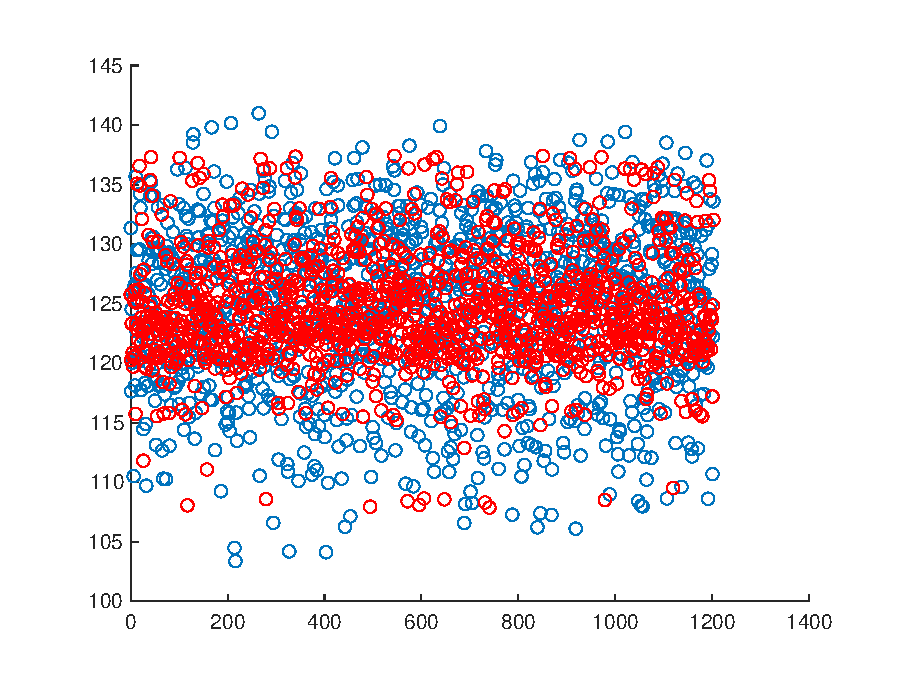
\includegraphics[width=\maxwidth{56.196688409433015em}]{figure_2.eps}
\end{center}
\begin{matlaboutput}
out = 5.8705e+03
\end{matlaboutput}
\begin{matlabcode}
[~, sorted_idx] = sort(fit0, 'ascend');
out=visucluster(cluster_pop{sorted_idx(1)},datatest,clusters)
\end{matlabcode}
\begin{center}
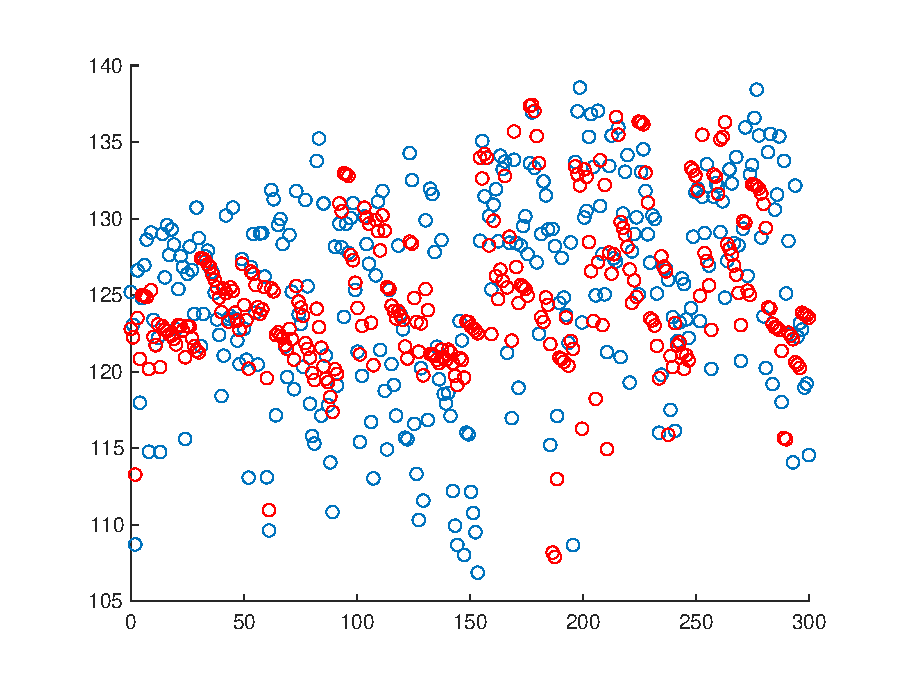
\includegraphics[width=\maxwidth{56.196688409433015em}]{figure_3.eps}
\end{center}
\begin{matlaboutput}
out = 1.4206e+03
\end{matlaboutput}
\begin{matlabcode}
figure;
plot(bestfit)
\end{matlabcode}
\begin{center}
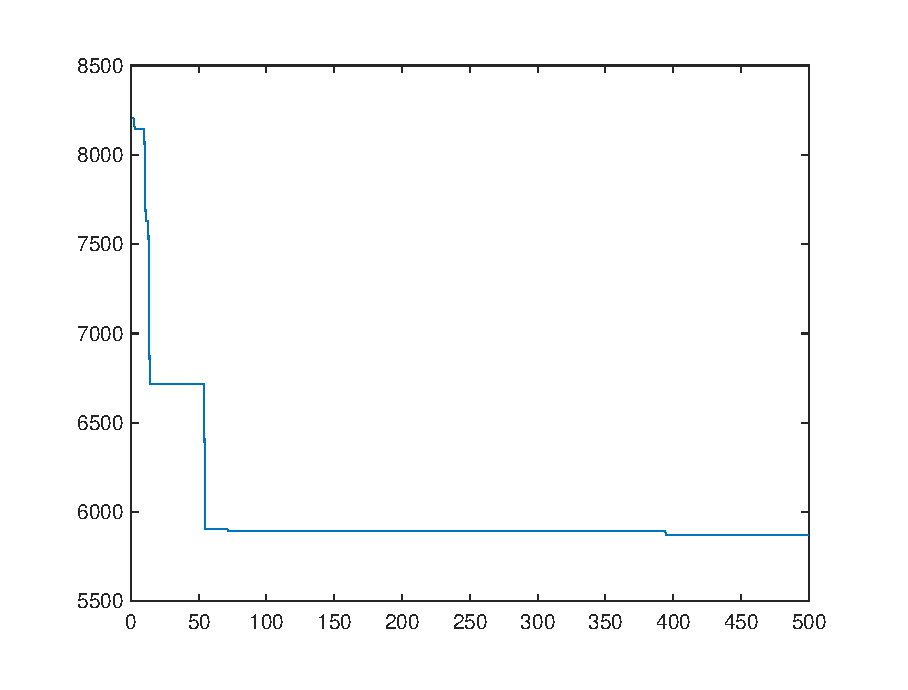
\includegraphics[width=\maxwidth{56.196688409433015em}]{figure_4.eps}
\end{center}

\begin{par}
\begin{flushleft}
here are all the functions used in the .mlx
\end{flushleft}
\end{par}

\begin{matlabcode}
% TSK initializations
%  real mf bounds : 0:20000; 0:25; 0:0.35; 0:75; 0:0.06; 
% syntetic mf : 0:1; 0:1; 0:1 /normalized value
function pop=initfcm(popsize,clusters)
    pop=cell(popsize,1);

    mfs=[];
    for i=1:popsize
        for k=1:max(size(clusters))
            rule_param=50*(rand(1,6)-0.5); % parameters between -10 and 10;
            rule_param(1,6)=120+100*(rand(1,1)-0.75); % constant between 70 and 170
            pop{i}=[pop{i}; mfs rule_param];
        end
    end


end





function pop=initcluster(popsize,clusters)
    pop=cell(popsize,1);
    % we will use a gaussian membership function based on the different
    % cluster centers and the optimization parameter will be the standard
    % deviation "std"

    % we then have a total of 5 std to tune plus 6 rule parameter per
    % cluster, totaling 11*13=143 parameters

    mfs=[];
    for i=1:popsize
        for k=1:max(size(clusters))
            mfs=0.05+0.15*rand(1,5); % initialize the std the between 0.05 and 0.1  for each cluster
            rule_param=20*(rand(1,6)-0.5); % parameters between -5 and 5;
            rule_param(1,6)=120+110*(rand(1,1)-0.5);
            pop{i}=[pop{i}; mfs rule_param];
        end
    end
end


%selection, mutation, reproduction
function [num_elites,pool] = selection(pop, fitness_vals, rate,popsize,e_rate)
    % popsize = length(pop);
    num_selected = round(rate * popsize);  
    num_elites = ceil(e_rate * popsize);
    [~, sorted_idx] = sort(fitness_vals, 'ascend');
    elites = pop(sorted_idx(1:num_elites));  % Preserve the best individuals
    if size(elites,1)~=1
        elites=elites';
    end
    % Tournament Selection (forces selection pressure)
    num_to_select = num_selected - num_elites;
    selected_individuals = cell(1, num_to_select);
    for i = 1:num_to_select
        % Pick 3 random individuals and select the best one
        candidates = randperm(popsize, 3);
        [~, best_idx] = min(fitness_vals(candidates));
        selected_individuals{i} = pop{candidates(best_idx)};
    end

    % Combine elites and selected individuals
    pool = [elites, selected_individuals];
end

function child = mutation(child, mutation_rate,clusters)
    if rand < mutation_rate
        if rand>0.66
            new_child=initfcm(1,clusters);
            child=new_child{1};
        else

            child=child.*(1+(0.4*rand(15,6)-0.5)); % up to +-20%
        end
    end
end

function new_pop = reproduction(pool, mutation_rate, popsize,num_elites,clusters)
    new_pop = cell(1, popsize);
    
    for i = 1:num_elites
        new_pop{i} = pool{i}; % Directly copy elite individuals
    end
    for i = num_elites+1:popsize
        parent1 = pool{randi(length(pool))}; %select parents
        parent2 = pool{randi(length(pool))};
        child=zeros(15,6);
        % we want to do crossover on each membership function by doing an
        % interpolation of the parents parameters and crossover on rules
        alpha=rand(1);
        beta=1-alpha;
        child=parent1*alpha+parent2*beta;
        % child(1:13,1:5)=parent1(1:13,1:5)*alpha + parent2(1:13,1:5)*beta;
        % child(1:8,:)= [parent1(1:8,:)];
        % child(9:15,:)=[parent2(9:15,:)];
        
        % Mutation
        child = mutation(child, mutation_rate,clusters);
        
        new_pop{i} = child;
    end
end
function f=fitfcm(chr,data,ccs)
    
    for ind=1:length(data)
        output=0;
        for k = 1:size(ccs,2)
            dist_ik = norm(data(ind,1:5) - ccs(k,:)) + 1e-6; % small value to avoid div by zero
            denom = 0;
            for j = 1:size(ccs,2)
                dist_ij = norm(data(ind,1:5) - ccs(j,:)) + 1e-6;
                denom = denom + (dist_ik / dist_ij)^(2/(2.5-1));
            end
            U_test(k) = 1 / denom;
            
            a = chr(k,1:5); % 5 coefficients
            b = chr(k,6);   % bias
            y_k = dot(a, data(ind,1:5)) + b;
            output = output + U_test(k) * y_k;
        end
        pred(ind,1) = output;
    end
    errors = abs(pred - data(:,6));
    f = sum(errors)+10*max(errors);


end

function mu=fcmeval(datatest, clusters, m)
    c = size(clusters, 1); % number of clusters
    n = size(datatest, 1); % number of data points
    U_test = zeros(c, n);
    output=0;
    for i = 1:n
        for k = 1:c
            dist_ik = norm(datatest(i,:) - clusters(k,:)) + 1e-6; % small value to avoid div by zero
            denom = 0;
            for j = 1:c
                dist_ij = norm(datatest(i,:) - clusters(j,:)) + 1e-6;
                denom = denom + (dist_ik / dist_ij)^(2/(m-1));
            end
            U_test(k,i) = 1 / denom;
        end
    end
end

function f=fitcm(chr,data,ccs)
   for ind=1:length(data)
       w=ones(max(size(ccs)),1);
        % let's compute the firing power of each rule
        for k=1:max(size(ccs))
            for input=1:5
                w(k)=w(k)*exp(-(data(ind,input)-ccs(k,input))^2/(2*chr(k,input)^2)); % based on gaussian membership 
            end
        end
        agregg=sum(w);
        output = 0;
        for k = 1:max(size(ccs))
            x_inputs = data(ind, 1:5);
            rule_params = chr(k, 6:11); % [a1...a5, b]
            rule_val = dot(rule_params(1:5), x_inputs) + rule_params(6);
            output = output + w(k) * rule_val;
        end
        pred(ind)=output/(agregg+10^(-10));
   end
   errors = abs(pred' - data(:,6));
   f = sum(errors);
end
% fitness function for 0 order tsk

function out=visu(chr, data,ccs)
    for ind=1:length(data)
       w=ones(max(size(ccs)),1);
        % let's compute the firing power of each rule
        for k=1:max(size(ccs))
            for input=1:5
                w(k)=w(k)*exp(-(data(ind,input)-ccs(k,input))^2/(2*chr(k,input)^2)); % based on gaussian membership 
            end
        end
        agregg=sum(w);
        output = 0;
        for k = 1:max(size(ccs))
            x_inputs = data(ind, 1:5);
            rule_params = chr(k, 6:11); % [a1...a5, b]
            rule_val = dot(rule_params(1:5), x_inputs) + rule_params(6);
            output = output + w(k) * rule_val;
        end
        pred(ind)=output/(agregg+10^(-10));
   end
   errors = abs(pred' - data(:,6));
   out = sum(errors);

    figure;
    scatter(linspace(0,length(data(:,6)),length(data(:,6))),data(:,6))
    hold on 
    scatter(linspace(0,length(data(:,6)),length(data(:,6))),pred,"red")

    % out=output;
end

function f=visucluster(chr,data,ccs)
    
    for ind=1:length(data)
        output=0;
        for k = 1:size(ccs,2)
            dist_ik = norm(data(ind,1:5) - ccs(k,:)) + 1e-6; % small value to avoid div by zero
            denom = 0;
            for j = 1:size(ccs,2)
                dist_ij = norm(data(ind,1:5) - ccs(j,:)) + 1e-6;
                denom = denom + (dist_ik / dist_ij)^(2/(2-1));
            end
            U_test(k) = 1 / denom;
            
            a = chr(k,1:5); % 5 coefficients
            b = chr(k,6);   % bias
            y_k = dot(a, data(ind,1:5)) + b;
            output = output + U_test(k) * y_k;
        end
        pred(ind,1) = output;
    end
    errors = abs(pred - data(:,6));
    f = sum(errors);

    figure;
    scatter(linspace(0,length(data(:,6)),length(data(:,6))),data(:,6))
    hold on 
    scatter(linspace(0,length(data(:,6)),length(data(:,6))),pred,"red")
end

\end{matlabcode}

\end{document}
